% Conceptual schematic; the label values illustrate C_8, not measured results.
% Styles adapted from the OpenResearch orx-tikz-preamble.tex scaffold.
% Single-column canvas: 86 mm = spconf column width ((178 mm - 6 mm) / 2).
% Include at width=\columnwidth (scale 1). Do not downscale fonts.
\documentclass[border=0pt]{standalone}
\usepackage[T1]{fontenc}
\usepackage{DejaVuSans}
\usepackage{tikz}
\usetikzlibrary{arrows.meta,positioning,calc}

\definecolor{orxblue}{HTML}{0072B2}
\definecolor{ink}{HTML}{17212B}
\definecolor{mutedink}{HTML}{5E6A75}
\tikzset{
  orx/.style={font=\sffamily\fontsize{9}{10.4}\selectfont,
    text=ink, line width=.9pt, >={Stealth[length=5.5pt,width=4.2pt,inset=1pt]}},
  heading/.style={font=\sffamily\fontsize{9.4}{11}\selectfont\bfseries,
    inner sep=0pt,align=left},
  label/.style={inner sep=0pt,align=center,text=mutedink},
  block/.style={draw=black!45,fill=black!2,rounded corners=1.2pt,line width=.8pt,
    minimum height=7.9mm,inner xsep=1.8pt,inner ysep=1.4pt,align=center},
  ours/.style={block,draw=orxblue,fill=orxblue!7,text=orxblue,line width=1.2pt},
  rating/.style={draw=black!45,fill=white,circle,line width=.8pt,
    minimum size=5.1mm,inner sep=0pt},
  flow/.style={->,draw=black!60,line width=.9pt},
  reveal/.style={->,draw=orxblue,line width=.9pt,dash pattern=on 3pt off 2pt},
}

\begin{document}
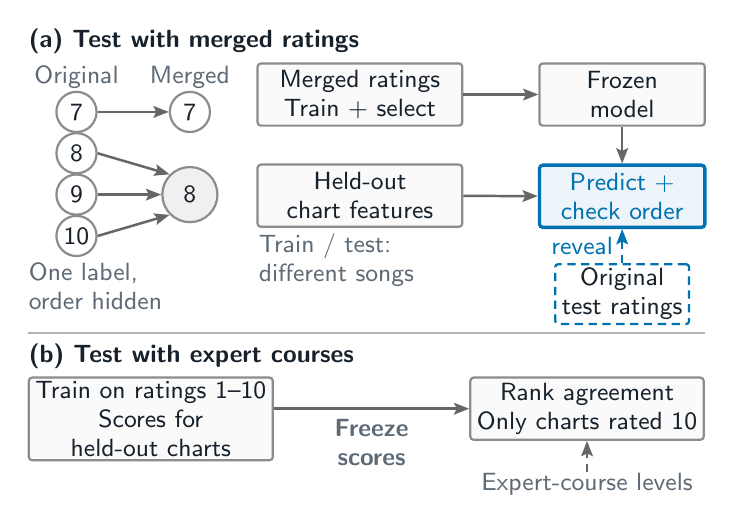
\begin{tikzpicture}[orx,x=1mm,y=1mm]
  % Fixed 86 mm width; the height follows the content.
  \path[use as bounding box] (0,0) rectangle (86,-59.6);

  % ---------------- (a) Test with merged ratings ----------------
  \node[heading,anchor=north west] at (0,0) {(a) Test with merged ratings};

  % Many distinct labels become the same observation. Item order is schematic.
  \node[label,anchor=north] (intact) at (6.2,-4.7) {Original};
  \node[label,anchor=north] (capped) at (20.6,-4.7) {Merged};
  \node[rating] (i7)  at (6.2,-10.7) {7};
  \node[rating] (i8)  at (6.2,-15.95) {8};
  \node[rating] (i9)  at (6.2,-21.2) {9};
  \node[rating] (i10) at (6.2,-26.45) {10};
  \node[rating] (c7)  at (20.6,-10.7) {7};
  \node[rating,minimum size=7mm,fill=black!6] (c8) at (20.6,-21.2) {8};
  \draw[flow] (i7) -- (c7);
  \draw[flow] (i8.east) -- (c8.north west);
  \draw[flow] (i9.east) -- (c8.west);
  \draw[flow] (i10.east) -- (c8.south west);
  \node[label,anchor=north west,align=left] (tie) at (0,-29.8)
    {One label,\\order hidden};

  % Fitting and outer-test evidence are visibly separated. There is no route
  % from intact test labels into fit/selection or the frozen model.
  \node[block,anchor=north,minimum width=26mm] (fit) at (42.2,-4.4)
    {Merged ratings\\Train + select};
  \node[block,anchor=north,minimum width=21mm] (frozen) at (75.5,-4.4)
    {Frozen\\model};
  \draw[flow] (fit) -- (frozen);
  \node[block,anchor=north,minimum width=26mm] (features) at (42.2,-17.25)
    {Held-out\\chart features};
  \node[ours,anchor=north,minimum width=21mm] (test) at (75.5,-17.25)
    {Predict +\\check order};
  \draw[flow] (features) -- (test);
  \draw[flow] (frozen) -- (test);
  \node[label,anchor=north west,align=left] (groups) at (29.2,-26.0)
    {Train / test:\\different songs};
  \node[draw=orxblue,line width=.8pt,dash pattern=on 3pt off 2pt,
    rounded corners=1pt,inner xsep=2.4pt,inner ysep=1.6pt,align=center,
    anchor=north] (answers) at (75.5,-29.9) {Original\\test ratings};
  \draw[reveal] (answers) -- node[label,left=1mm,text=orxblue] {reveal} (test);

  % Separator: the two tests share no edge.
  \draw[black!30,line width=.6pt] (0,-38.8) -- (86,-38.8);

  % ---------------- (b) Test with expert courses ----------------
  % This is a separate native-scale fit: no edge joins the two panels.
  \node[heading,anchor=north west] at (0,-40.0) {(b) Test with expert courses};
  \node[block,anchor=north west,inner xsep=2.4pt] (native) at (0,-44.3)
    {Train on ratings 1--10\\Scores for\\held-out charts};
  \node[block,anchor=north east,inner xsep=2.4pt] (agreement) at (86,-44.3)
    {Rank agreement\\Only charts rated 10};
  \draw[flow] (native.east |- agreement.west) -- (agreement.west)
    node[midway,below=1.2mm,label,align=center,
      font=\sffamily\fontsize{9}{10.4}\selectfont\bfseries] (freeze)
    {Freeze\\scores};
  \node[label,anchor=south] (tiers) at (agreement.south |- 0,-59.6)
    {Expert-course levels};
  \draw[flow,dash pattern=on 3pt off 2pt] (tiers) -- (agreement);
\end{tikzpicture}
\end{document}
